%----------------------------------------------------------------------------------------
%	PACKAGES AND OTHER DOCUMENT CONFIGURATIONS
%----------------------------------------------------------------------------------------

\documentclass[12pt]{article}
\usepackage[english]{babel}
%\usepackage[utf8x]{inputenc}
\usepackage[utf8]{inputenc}
\usepackage{amsmath,amsthm,amssymb}
\usepackage{bm}
\usepackage{graphicx}
\usepackage[colorinlistoftodos]{todonotes}
\usepackage{pythonhighlight}
\usepackage{placeins}
\usepackage{chngcntr}
\counterwithin{figure}{section}
\usepackage{indentfirst}
\usepackage{xfrac}
\usepackage{textcomp}
\usepackage[linesnumbered,ruled,vlined]{algorithm2e}
\usepackage{algorithmic}
\usepackage{graphicx}
\usepackage{subfigure}
\setlength{\parindent}{2em}
% caption space control
%\usepackage[belowskip=-13pt,aboveskip=0pt,font=small,labelfont=bf]{caption}
%\usepackage[font=small,labelfont=bf]{caption}
% caption and subcaption work together
\usepackage{enumitem}
\newlist{steps}{enumerate}{1}
\setlist[steps, 1]{label = Step \arabic*:}
% Step env
\usepackage{caption}
% \usepackage{subcaption}
% Here: H option for float placement
\usepackage{float}
% comment block
\usepackage{verbatim}
%hyperlink
\usepackage{hyperref}
\usepackage[title]{appendix}  
\usepackage{diagbox}
\usepackage{booktabs}
%Times new roman
%https://liam.page/2017/01/10/Times-New-Roman-and-LaTeX/
\usepackage[T1]{fontenc}
\usepackage{mathptmx}
% File Structure
\usepackage{dirtree}
\usepackage{xcolor}
% The following is a dummy icon command
\newcommand\myicon[1]{{\color{#1}\rule{2ex}{2ex}}}
% If you have actual icon images, use \includegraphics to include them
% If you are generating them, put in the appropriate code for them here
% now we make a command for a folder/file which inserts the icon and its label
% adjust this as needed. If you only have 2 icons, then you could create
% a \myfile and \myfolder command with the icon fixed.
\newcommand{\myfolder}[2]{\myicon{#1}\ {#2}}


\usepackage{pdfpages}

\usepackage{biblatex}
%\usepackage[square,sort&compress,numbers]{natbib}
%\bibliographystyle{acm}
%\bibliography{references}
\addbibresource{references.bib}

\newcommand{\N}{\mathbb{N}}
\newcommand{\Z}{\mathbb{Z}}
\newcommand{\R}{\mathbb{R}}
\newcommand{\X}{\mathbb{X}}
\DeclareMathAlphabet{\pazocal}{OMS}{zplm}{m}{n}

\newtheorem{theorem}{Theorem}[section]
\newtheorem{lemma}[theorem]{Lemma}
\newtheorem*{remark}{Remark}
\newtheorem{problem}{Problem}
\begin{document}

\begin{titlepage}

\newcommand{\HRule}{\rule{\linewidth}{0.5mm}} % Defines a new command for the horizontal lines, change thickness here

\center % Center everything on the page
 
%----------------------------------------------------------------------------------------
%	HEADING SECTIONS
%----------------------------------------------------------------------------------------

\includegraphics[width=0.25\textwidth]{fig/aalto_logo.png}

\textsc{\LARGE Aalto University}\\[2 cm]

\textsc{\LARGE Research Project Report}\\[0.3cm] % Name of your university/college
 % Minor heading such as course title

%----------------------------------------------------------------------------------------
%	TITLE SECTION
%----------------------------------------------------------------------------------------

\HRule \\[0.4cm]
{ \huge Applying Gaussian Processes to High Frequency Trading}\\[0.4cm]
%{ \large \textbf{Diagnosis and theranostics by applied machine learning methods to metabolomic data.}  }\\[0.15cm] % Title of your document
\HRule \\[0.4cm]
 
%----------------------------------------------------------------------------------------
%	AUTHOR SECTION
%----------------------------------------------------------------------------------------


{\raggedright
\textbf{Chengyu \textsc{Hao}, Yaowei \textsc{LI}} - Data Science(EIT digital), School of computer science, Aalto University \\
Research Project 
\\[3mm]}


\textbf{\emph{Supervisors:}} \\[2mm]
{\raggedright
\textbf{\textsc{Paul Chang, Arno Solin}} - School of Computer Science, Aalto University\\[1mm]
}
% If you don't want a supervisor, uncomment the two lines below and remove the section above
%\Large \emph{Author:}\\
%John \textsc{Smith}\\[3cm] % Your name

%----------------------------------------------------------------------------------------
%	DATE SECTION
%----------------------------------------------------------------------------------------

 % Date, change the \today to a set date if you want to be precise
 %{\raggedright\\[1cm]}

%----------------------------------------------------------------------------------------
%	LOGO SECTION
%----------------------------------------------------------------------------------------

% Include a department/university logo - this will require the graphicx package
 
%----------------------------------------------------------------------------------------


\vfill % Fill the rest of the page with whitespace

\end{titlepage}

\setcounter{page}{1}
\pagenumbering{roman}
\tableofcontents
\pagebreak

\setcounter{page}{1}
\pagenumbering{arabic}

\section{Introduction}
High Frequency trading (HFT) is applied as a platform for matching buyers and sellers in financial asset markets. The transactional data captured can be thought of as an unbounded time series. Recent advances in theory allow for Gaussian Processes to predict online and inference for otherwise computationally infeasible applications. However, the time complexity of fitting the Gaussian process is cubic time complexity, which is impossible to be implement in the high frequency trading. In order to fit the HFT data in linear time, we need to identify a new method that can fit the data more efficiently. \\

The Kalman filter algorithm applies the concept of state space, based on time domain design, is a highly efficient recursive filter (autoregressive filter) that can be applied from a series of incomplete and noise-containing measurements. It estimates the state of the dynamic system and reduces the algorithm time and space complexity, and is widely used in various signal estimation.\\

In this report, we show how temporal Gaussian process regression models in machine learning can be reformulated as linear-Gaussian state space models, which can be solved exactly with classical Kalman filtering theory. The result is an efficient non-parametric learning algorithm, whose computational complexity grows linearly with respect to number of observations. We use this method to online predict the HFT process. Specifically, the method in this report involves: 1. extracting information representations of HFT data that optimally represents market dynamics; 2. compare the Gaussian process with different time series forecasting models on HFT data, like ARIMA, and evaluate the performance; 3. transfer the Gaussian process model to state space model to allow for linear time complexity, and use automatic pattern discovery kernels to achieve better fitting and predicting results.


\section{Data Description}
In order to get the reliable and true HFT dataset, we used the dataset downloaded from FXCM. FXCM is a leading provider of online foreign exchange (FX) trading, CFD trading, spread betting and related services. FXCM provides a API called FXCMPY to interact with its trading platform. Basically, it allows the retrieval of historical data as well as of streaming data. In addition, it allows to place different types of orders and to read out account information. \\

In this report, we downloaded HFT dataset from FXCM with different frequencies and different kind of foreign exchange, the minimum frequency is 1 min. Figure 2.1 shows the example of different foreign exchange for "bidopen" dataset with sampling frequency as 1 min. In this example, we retrieve 100 data points for each kind of foreign exchange, and the date is 11/19/2019. 


\begin{figure}[H]
\subfigure[USD/CAD]{\label{fig:a}
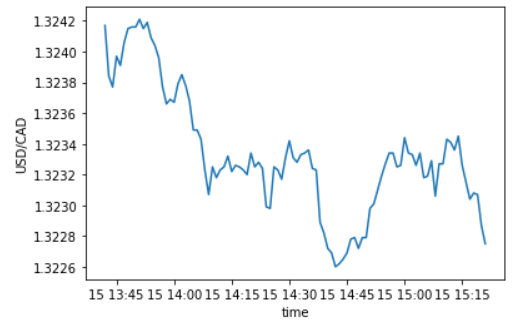
\includegraphics[width=6cm]{fig/section2/USDCAD.PNG}
}
\subfigure[USD/CHN]{\label{fig:b}
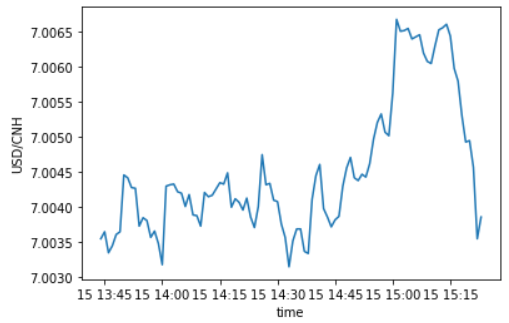
\includegraphics[width=6cm]{fig/section2/USDCHN.PNG}
}

\subfigure[EUR/USD]{\label{fig:a}
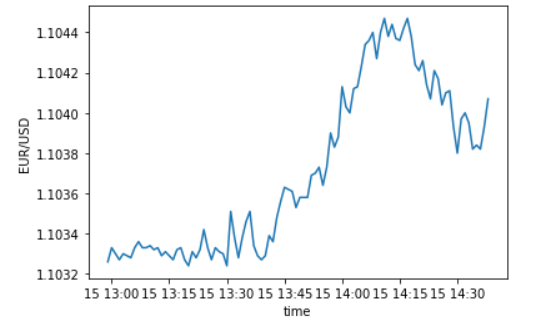
\includegraphics[width=6cm]{fig/section2/usdeur.PNG}
}
\subfigure[USD/JPY]{\label{fig:a}
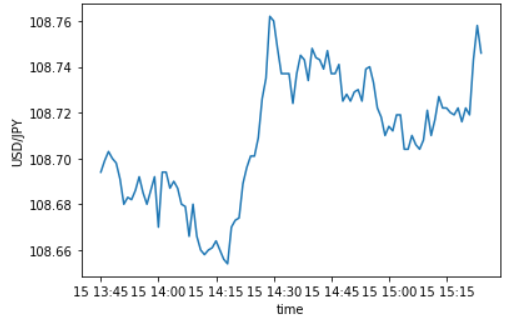
\includegraphics[width=6cm]{fig/section2/USDJPY.PNG}
}
\caption{the relationship between time and exchange rate for different currencies with 1-min frequency}
\end{figure}

\section{Compare Gaussian Process with Different Time Series Forecasting Models}
\subsection{ARIMA}
ARIMA is an acronym that stands for AutoRegressive Integrated Moving Average. It is a generalization of the simpler AutoRegressive Moving Average and adds the notion of integration. This acronym is descriptive, capturing the key aspects of the model itself. Briefly, they are:\\

AR: Autoregression. A model that uses the dependent relationship between an observation and some number of lagged observations.\\

I: Integrated. The use of differencing of raw observations (e.g. subtracting an observation from observation at the previous time step) to make the time series stationary.\\

MA: Moving Average. A model that uses the dependency between an observation and a residual error from a moving average model applied to lagged observations.\\

Each of these components is explicitly specified in the model as a parameter. Standard notation is used of ARIMA(p,d,q) where the parameters are substituted with integer values to quickly indicate the specific ARIMA model being used.\\

The parameters of the ARIMA model are defined as follows:\\

p: The number of lag observations included in the model, also called the lag order.\\

d: The number of times that the raw observations are differenced also called the degree of differencing.\\

q: The size of the moving average window, also called the order of moving average.

\subsubsection{ARIMA Parameters}
Firstly, we need to select the value of d. We can see from figure 1 that the dataset is not that stationary, this suggests that the time series will require differencing to make it stationary, at least a differencing order of 1. Figure 2 shows the time series of figure 1 with differencing as 1, it is clear that the time series become more stationary, so we choose the value of d as 1.

\begin{figure}[H]
\centering 
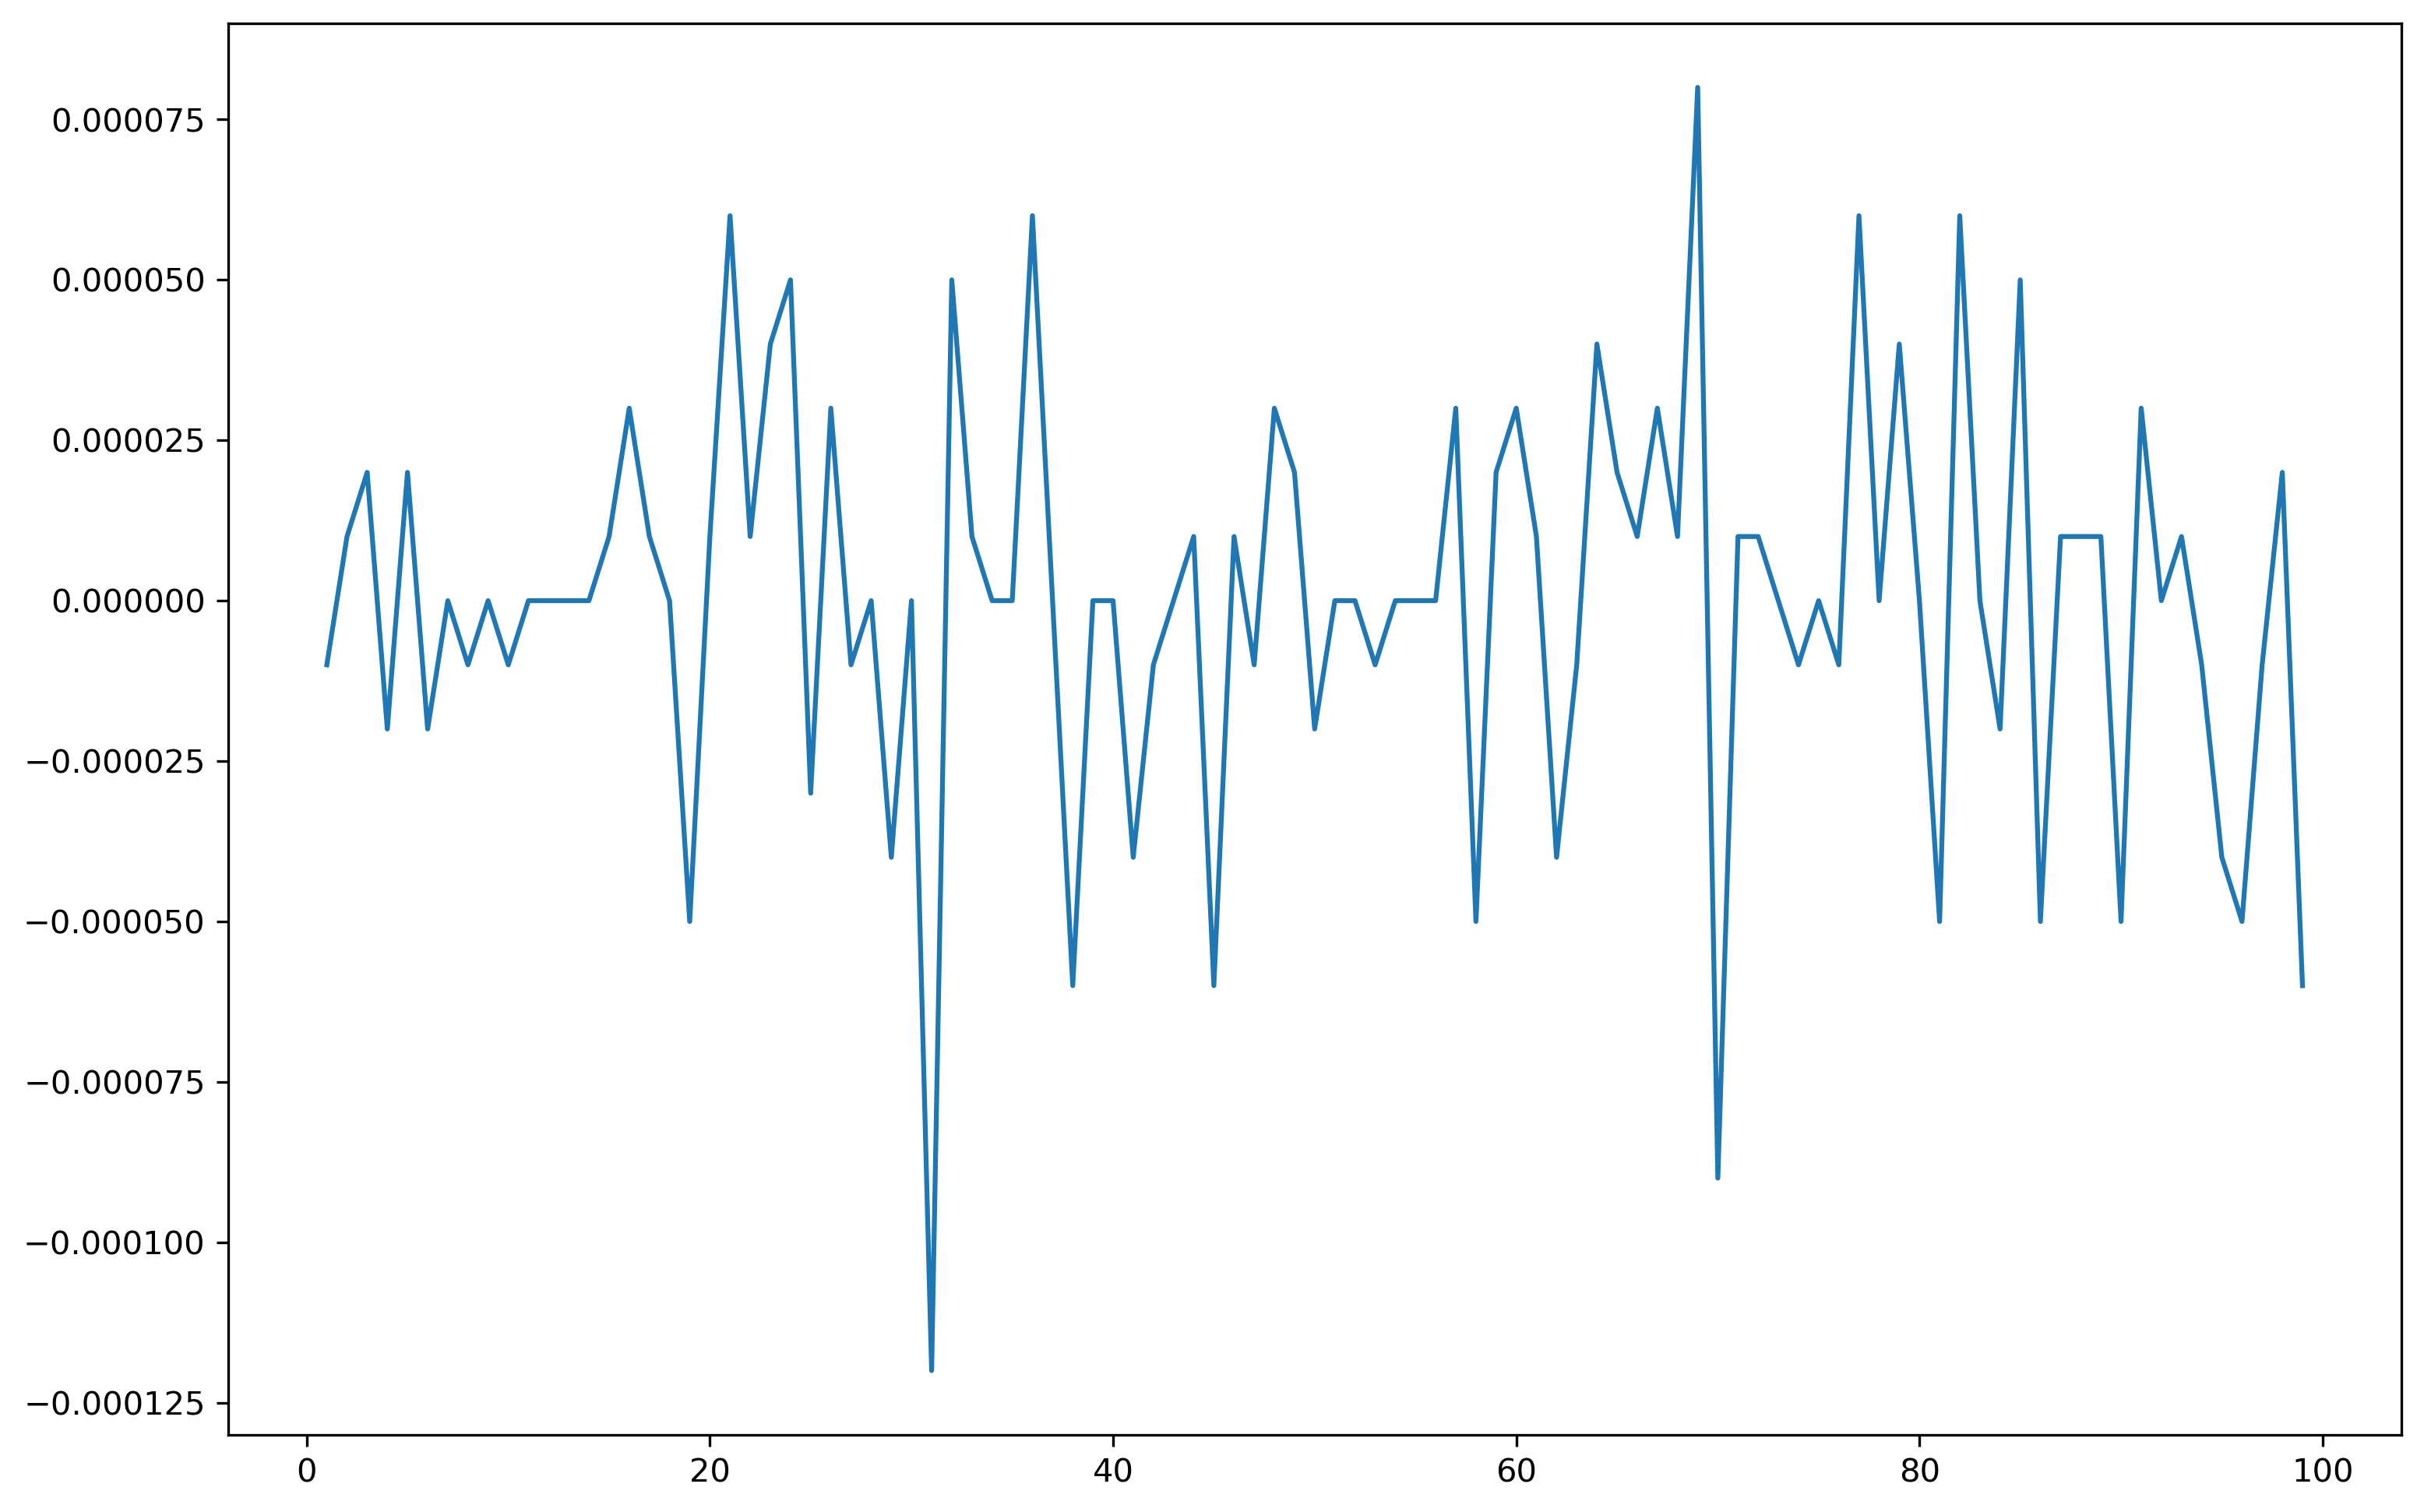
\includegraphics[width=0.7\textwidth]{fig/section3/m1_400to500_diff1.png}
\centering 
\caption{The grammar definition.}
\label{fig:grammar}
\end{figure}

\begin{figure}[H]
\centering 
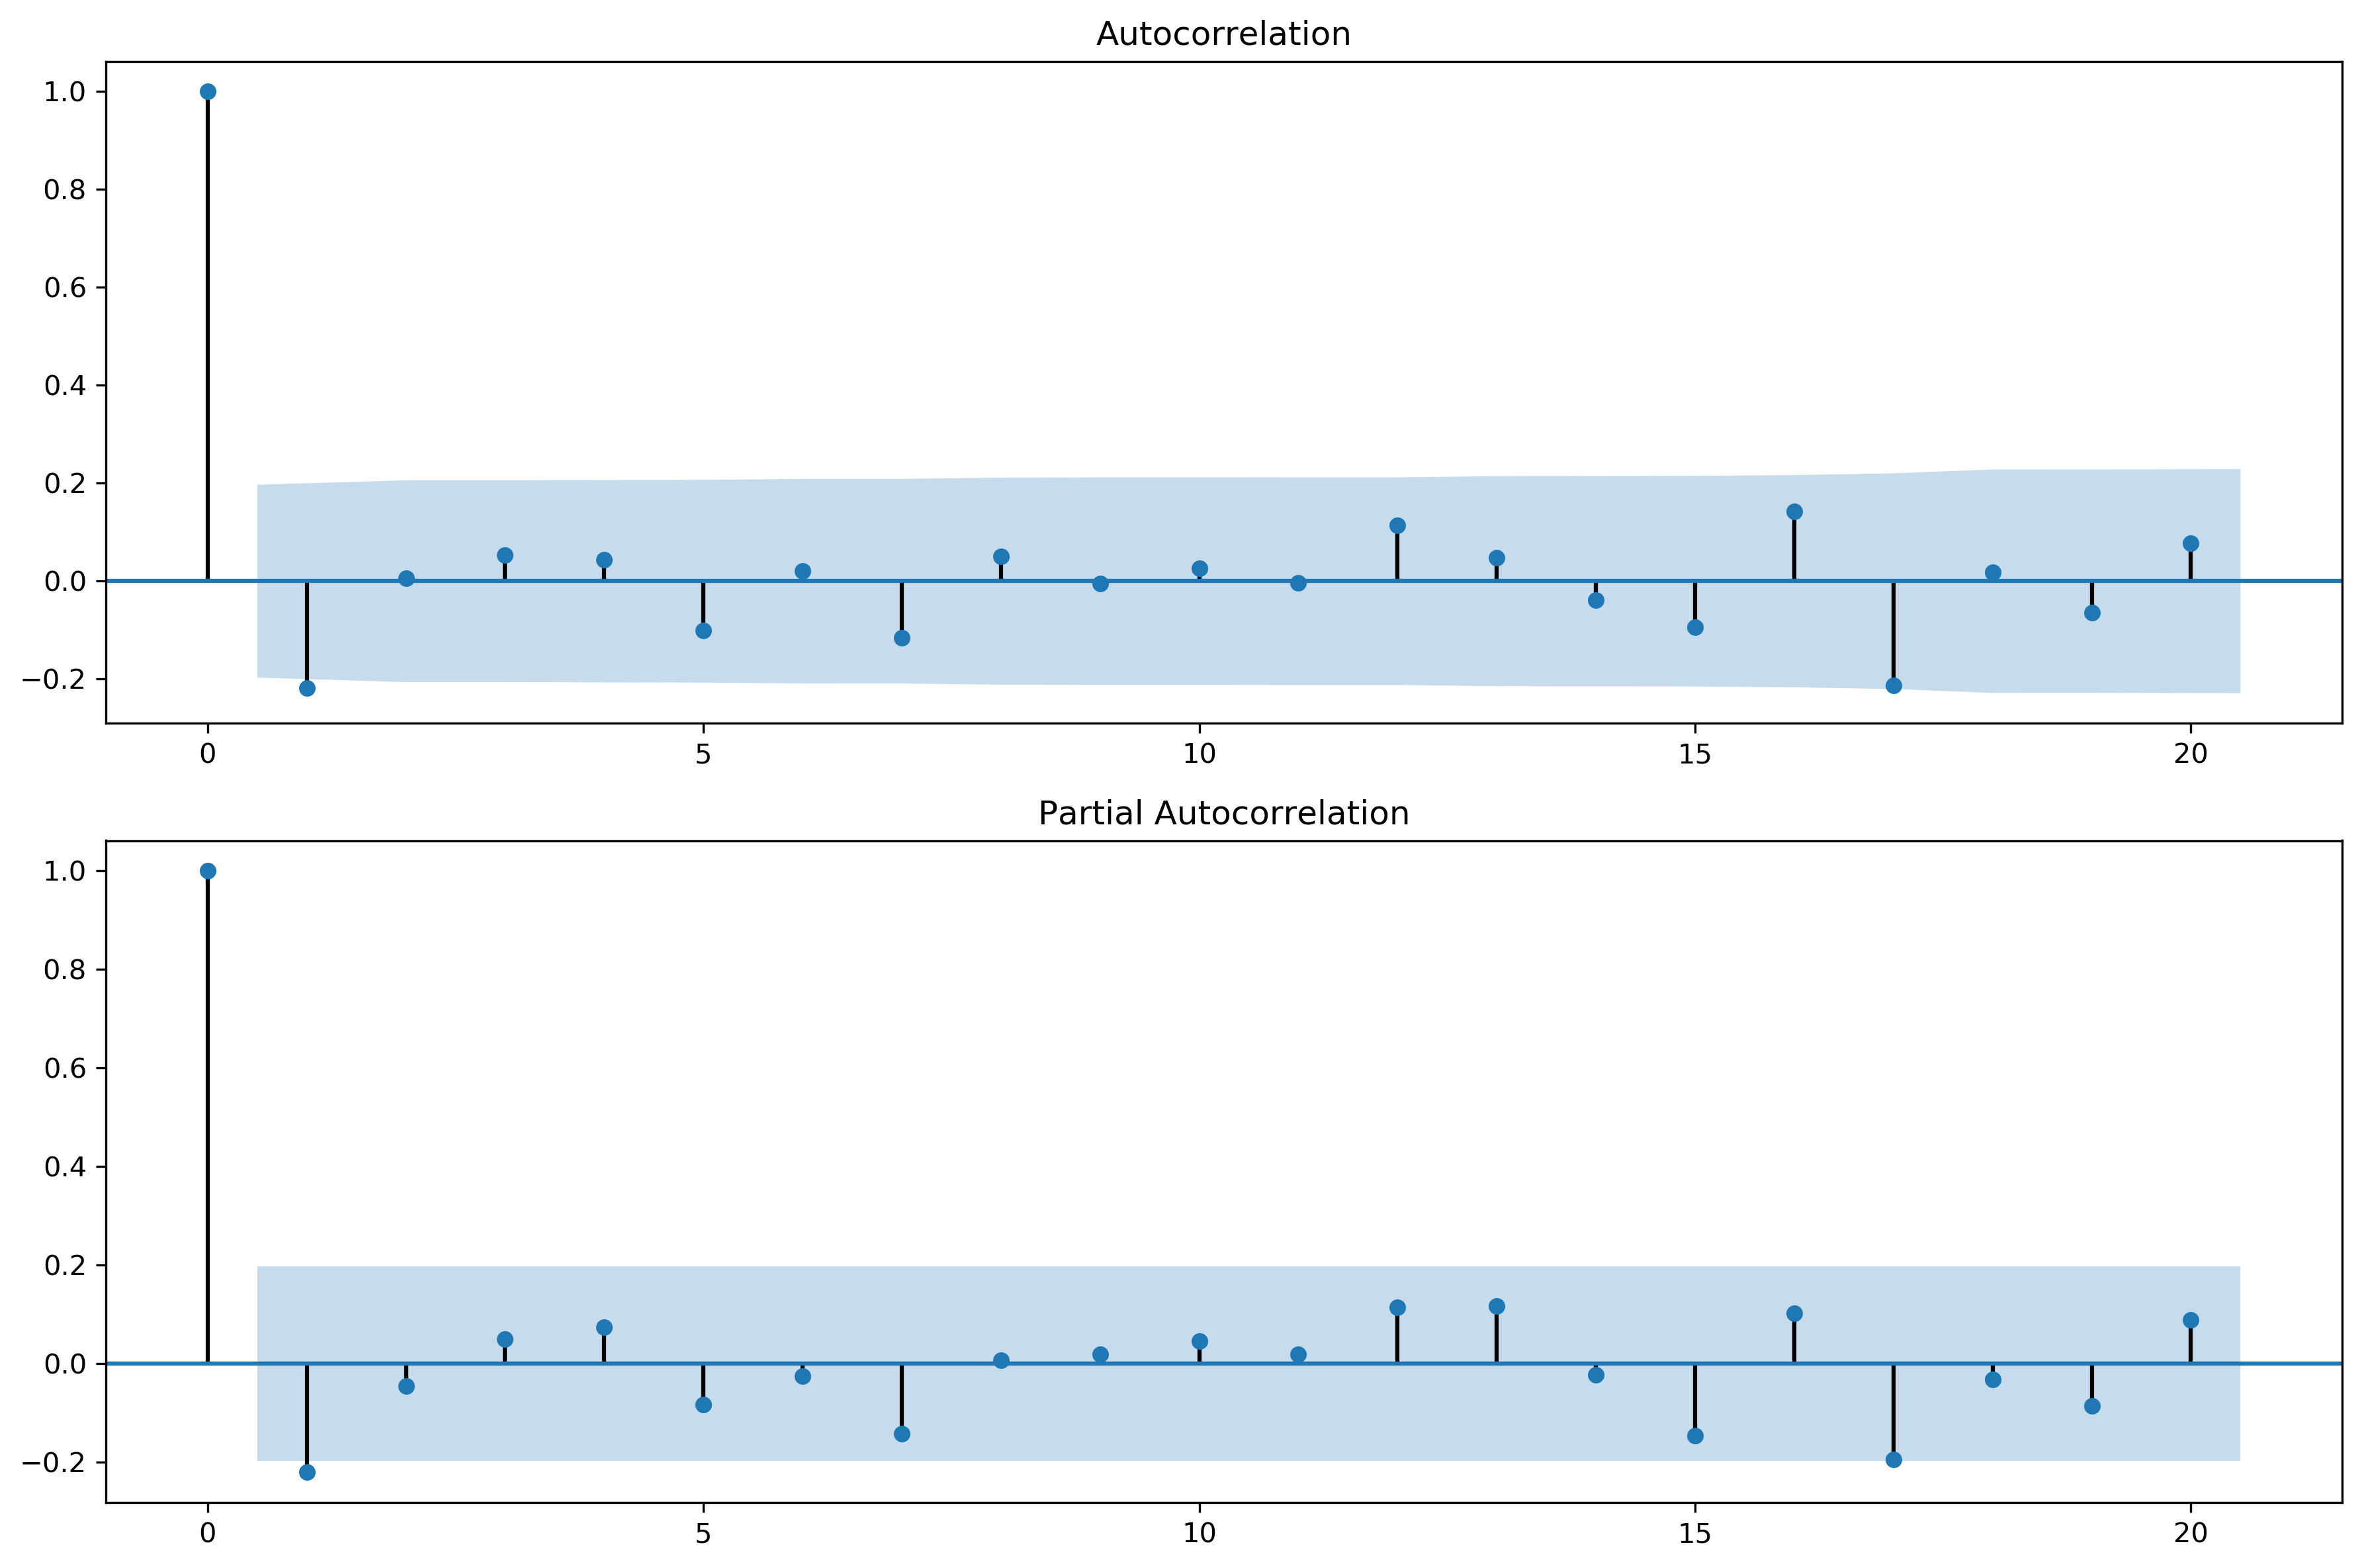
\includegraphics[width=0.7\textwidth]{fig/section3/m1_400to500_choose_parameters.png}
\centering 
\caption{"bidopen" dataset with sampling frequency as 1 min and differencing as 1}
\label{fig:grammar}
\end{figure}

For the parameters of p and q, the easiest way to choose them is using the autocorrelation and partial autocorrelation figure. Figure 3 is the autocorrelation and partial autocorrelation of the time series in figure 2. We use the autocorrelation figure to decide the value of q and partial autocorrelation figures to decide the value of p. According to figure 3, after p = 1, all partial autocorrelation values fall within the confidence interval, so we choose p = 1, the same as the choice of q.\\

After the choice of p, d, and q, we can fit an ARIMA(1,1,1) model for the dataset with frequency as 1 min. This model sets the lag value to 1 for autoregression, uses a difference order of 1 to make the time series stationary, and uses a moving average model of 1.

\subsection{Gaussian process}

We try different kernels to fit the data. Several kernels are considered below:
\begin{itemize}
    \item Polynomial kernel.
    The Polynomial kernel is defined as:
$$k(x,y)=(x^T*y+c)^d$$

\item Periodic kernel.
The Periodic kernel is defined as:
$$ k(x,y) = \theta_1 \exp \left[  - \frac{1}{2} \sum_{i=1}^{input\_dim}
       \left( \frac{\sin(\frac{\pi}{T_i} (x_i - y_i) )}{l_i} \right)^2 \right]$$
       
\item RBF kerne:
$$k(r) = \sigma^2 \exp \bigg(- \frac{1}{2} r^2 \bigg)$$
    
\item linear kernel:
$$k(x,y) =\sum_{i=1} ^{input\_dim}\sigma^2_i x_iy_i$$

\end{itemize}

We combined different kernels with the period kernel, in total, we have three different kernels in our experiment: Periodic+Liner kernel, Periodic+RBF kernel, and Periodic+poly kernel.


\subsection{Experimental Setup}
We fixed the currency as USD-EUR, and choose 4 kinds of time frequency (m1, m5, m30, h4) to evaluate the model performance under different time frequency. \\

We use a walk-forward validation method to evaluate model performance. Every time one test data point will be predicted by the model, and then the model will shift forward and include the data point in the test set that we used before. For example, we set the training dataset from point 1 to point 89, and then predict the points 90, and then we set the training dataset from point 1 to point 90, and then predict the points 91, this process repeats until the test set are all evaluated. Also, the move stride can not only be 1. For example, We can set the stride as 10, and the training dataset from point 1 to point 80, and then predict the point 90, and then move forward. Finally, we use the true value of the test set to compare to the predicted value. In our experiment, the stride is set to be 1 and 10. \\

For the measuring metrics, two methods are commonly used to evaluate the set, and those are the mean squared error (MSE) and the mean absolute error (MAE), the definition is shown below. MSE computes the mean of the squared error over the error set, while the MAE calculates the mean of the absolute error.  Both MSE and MAE have the benefit of removing the difference between negative and positive errors, and one difference between MSE and MAE is that the MSE is more reactive to extreme errors because of the square operation. In our experiment, we use MAE as our metric.

 \begin{align*}
&MSE\ =\ \frac{1}{n}\sum ^{n}_{i=1}\left( y_{i} -y^{*}_{i}\right)^{2}\\
&MAE\ =\ \frac{1}{n}\sum ^{n}_{i=1} |y_{i} -y^{*}_{i} |
 \end{align*}
 
\subsection{Result}
In our experiment, we have 4 models in total: ARIMA model and 3 GP model with kernels as Periodic+Liner kernel, Periodic+RBF kernel, and Periodic+poly kernel.\\

Firstly, we use the stride as 1 and evaluated 4 datasets with all the models. We use MAE as our metric, and compare the MAE among all these models. Figure 4 - figure 7 is the predicted results using walk-forward validation for 10 data points. The light blue line is the true data, the red line corresponded to the ARIMA model, the blue, green and cyan lines corresponded to Periodic+Liner kernel, Periodic+RBF kernel, and Periodic+poly kernel models, respectively. The MAE results are shown in Table 1. We found that for all the frequencies, we can always find at least one GP model which performs better than ARIMA model, this result reveals that GP model is more flexible than ARIMA model, since the GP model can choose different kernels to adapt to the dataset.



\begin{figure}[H]
\centering 
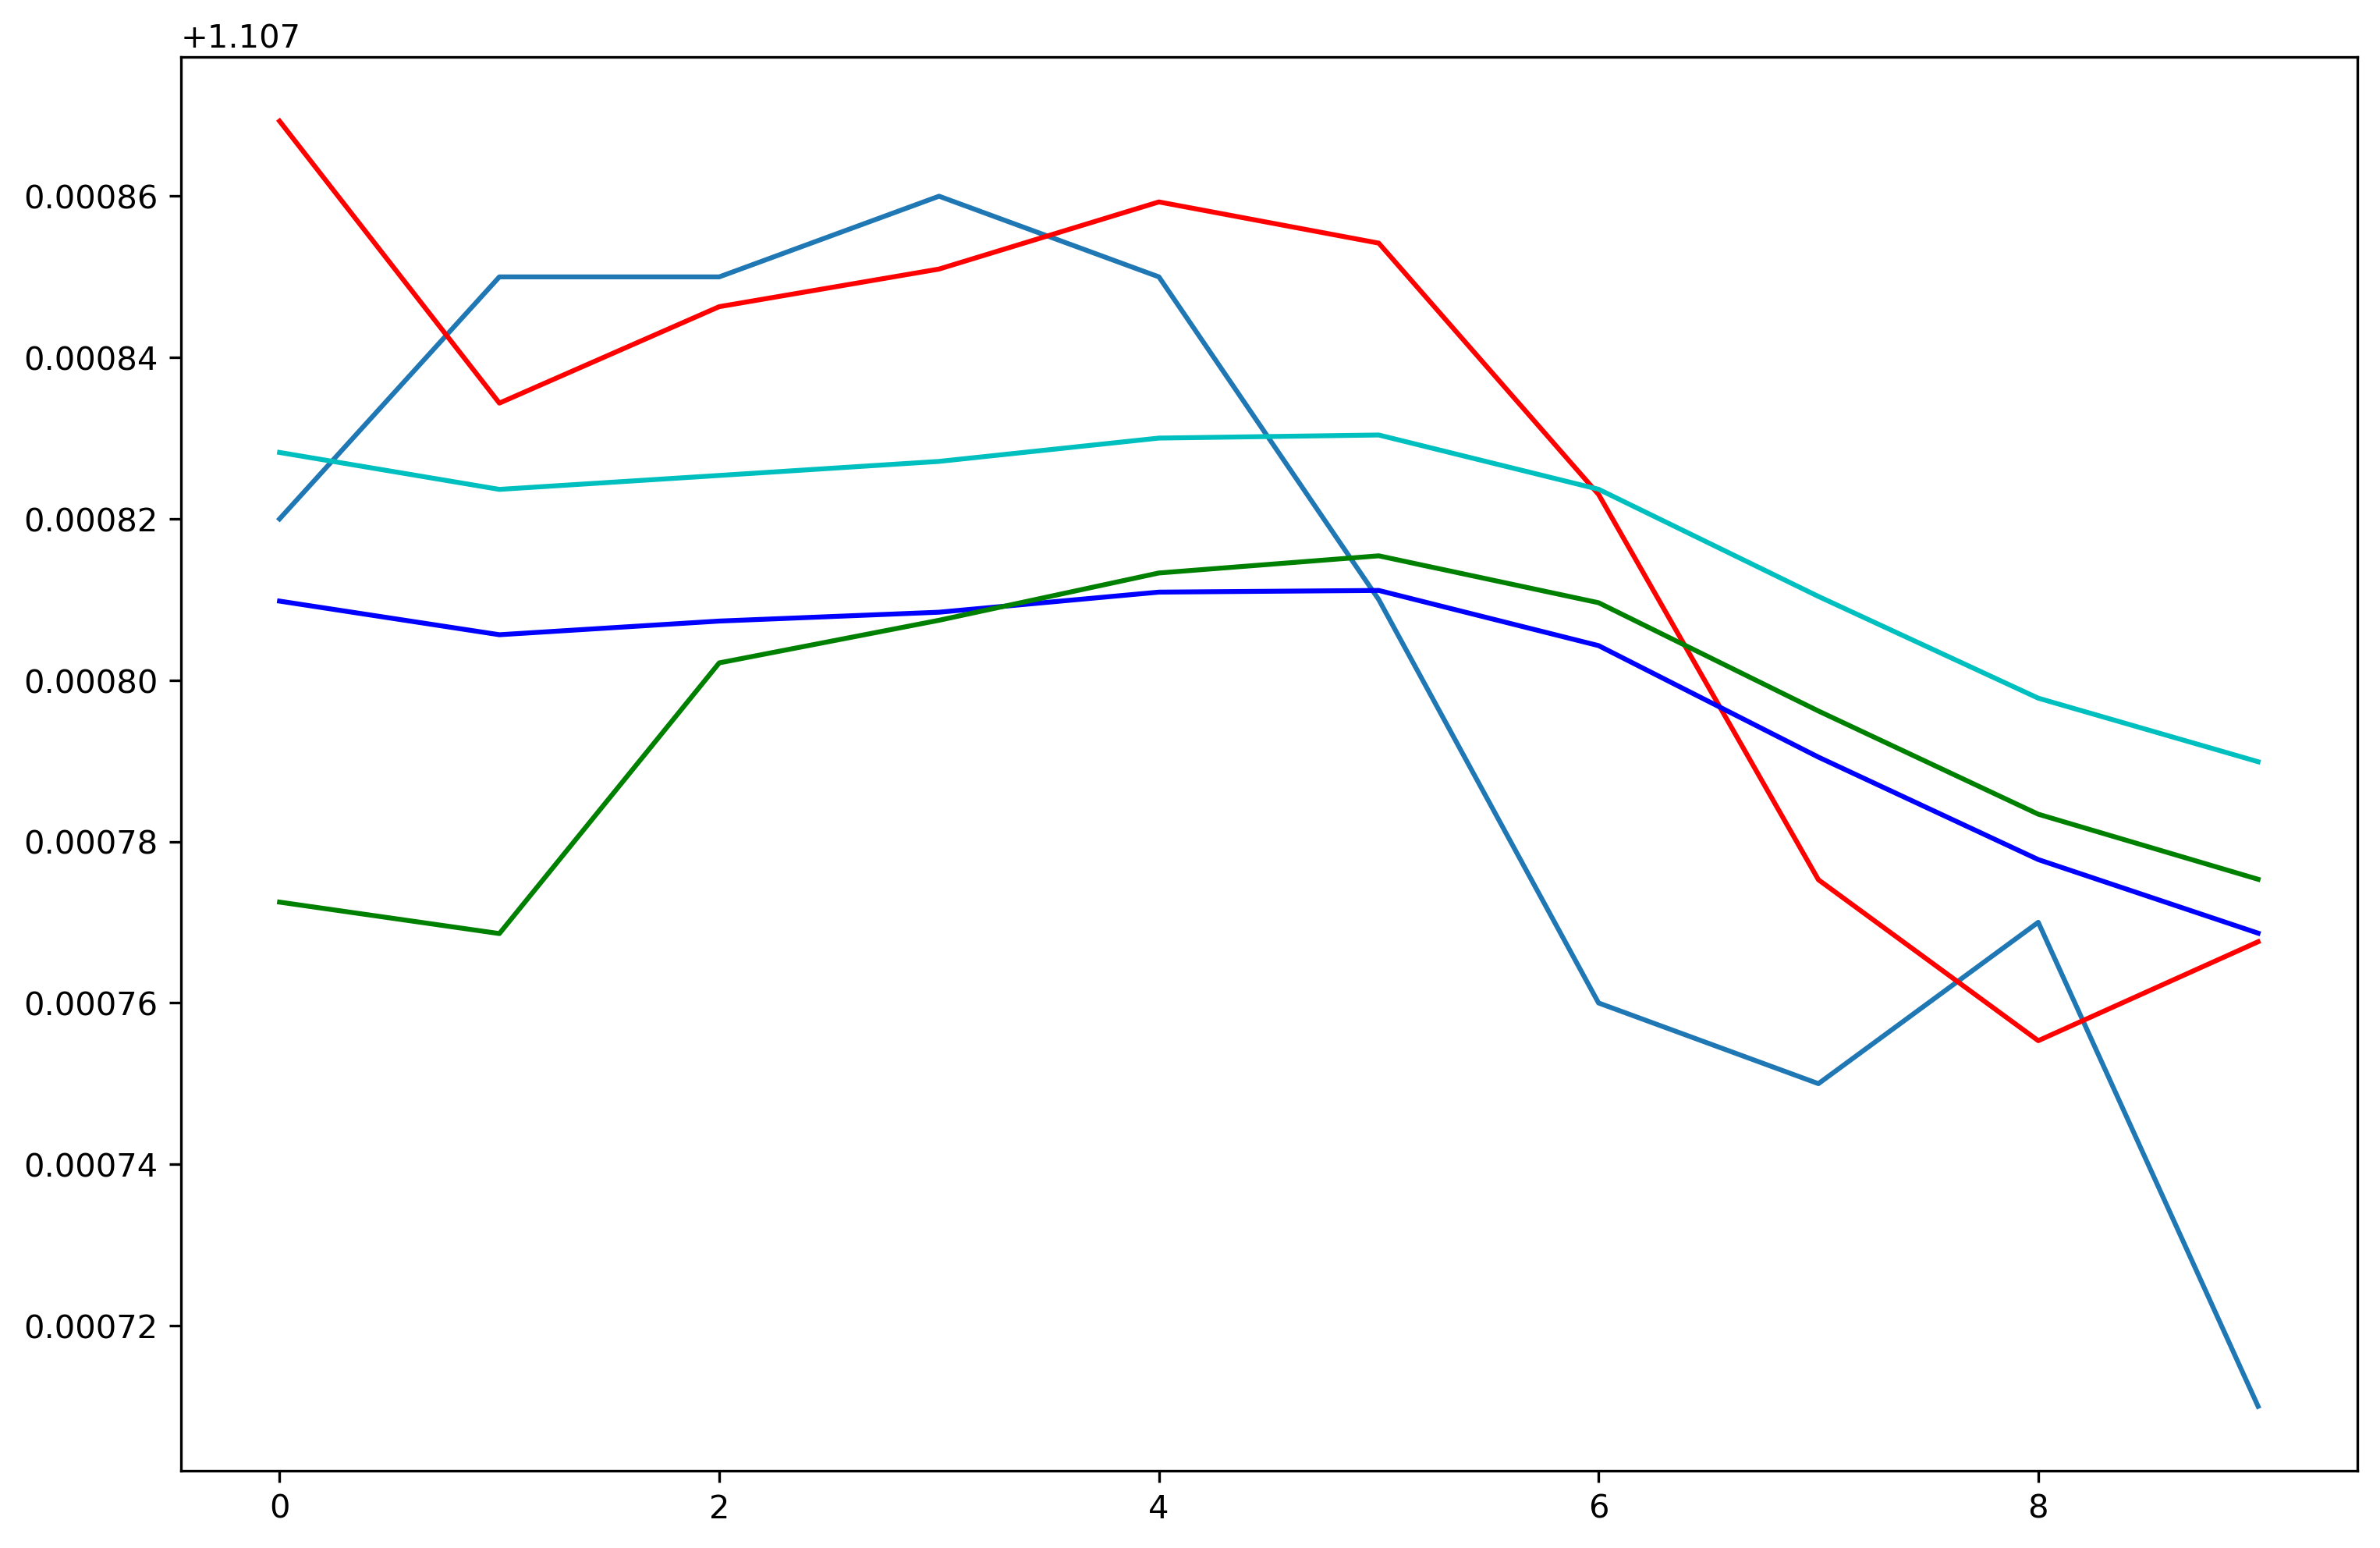
\includegraphics[width=0.7\textwidth]{fig/section3/m1_h1_all_together.png}
\centering 
\caption{Predicted result of last 10 data points with sampling frequency as 1 min and stride as 1. The light blue line is the true data point, the red line corresponded to the predicted result of ARIMA model, the blue, green and cyan lines corresponded to the predicted results of Periodic+Liner kernel, Periodic+RBF kernel, and Periodic+poly kernel models. }
\label{fig:grammar}
\end{figure}

\begin{figure}[H]
\centering 
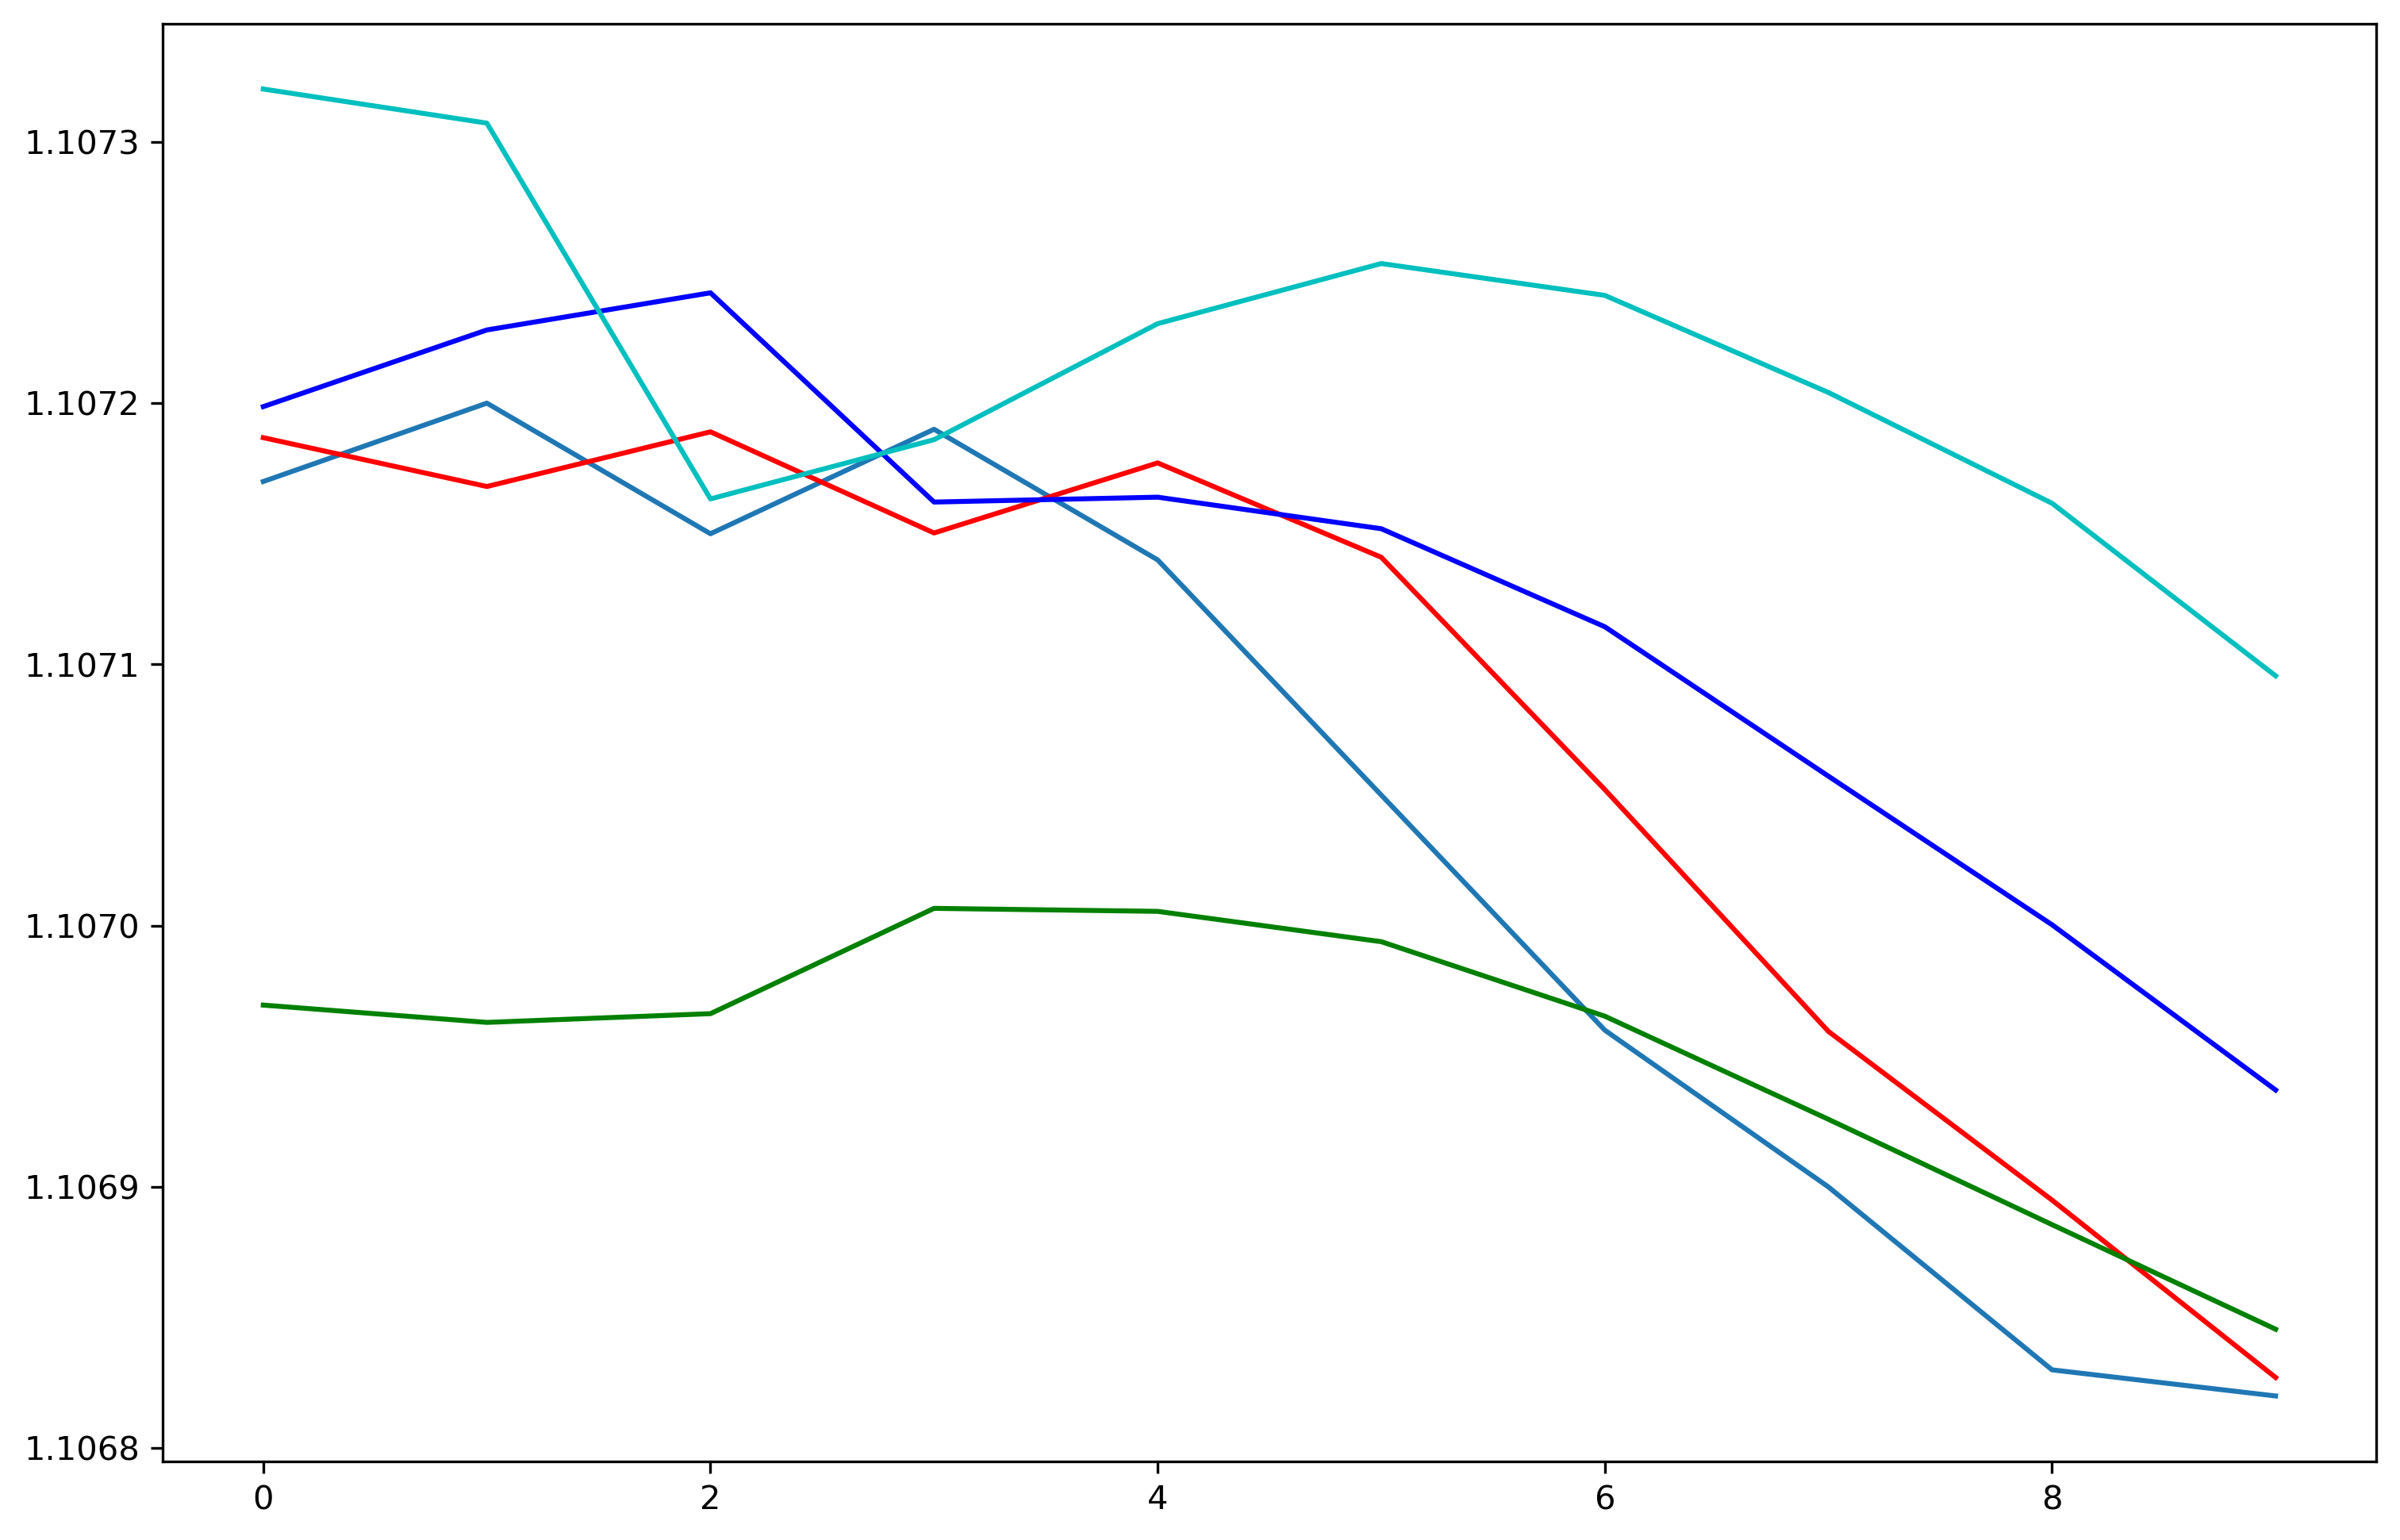
\includegraphics[width=0.7\textwidth]{fig/section3/m5_h1_all_together.png}
\centering 
\caption{Predicted result of last 10 data points with sampling frequency as 5 min and stride as 1. The light blue line is the true data point, the red line corresponded to the predicted result of ARIMA model, the blue, green and cyan lines corresponded to the predicted results of Periodic+Liner kernel, Periodic+RBF kernel, and Periodic+poly kernel models.}
\label{fig:grammar}
\end{figure}


\begin{figure}[H]
\centering 
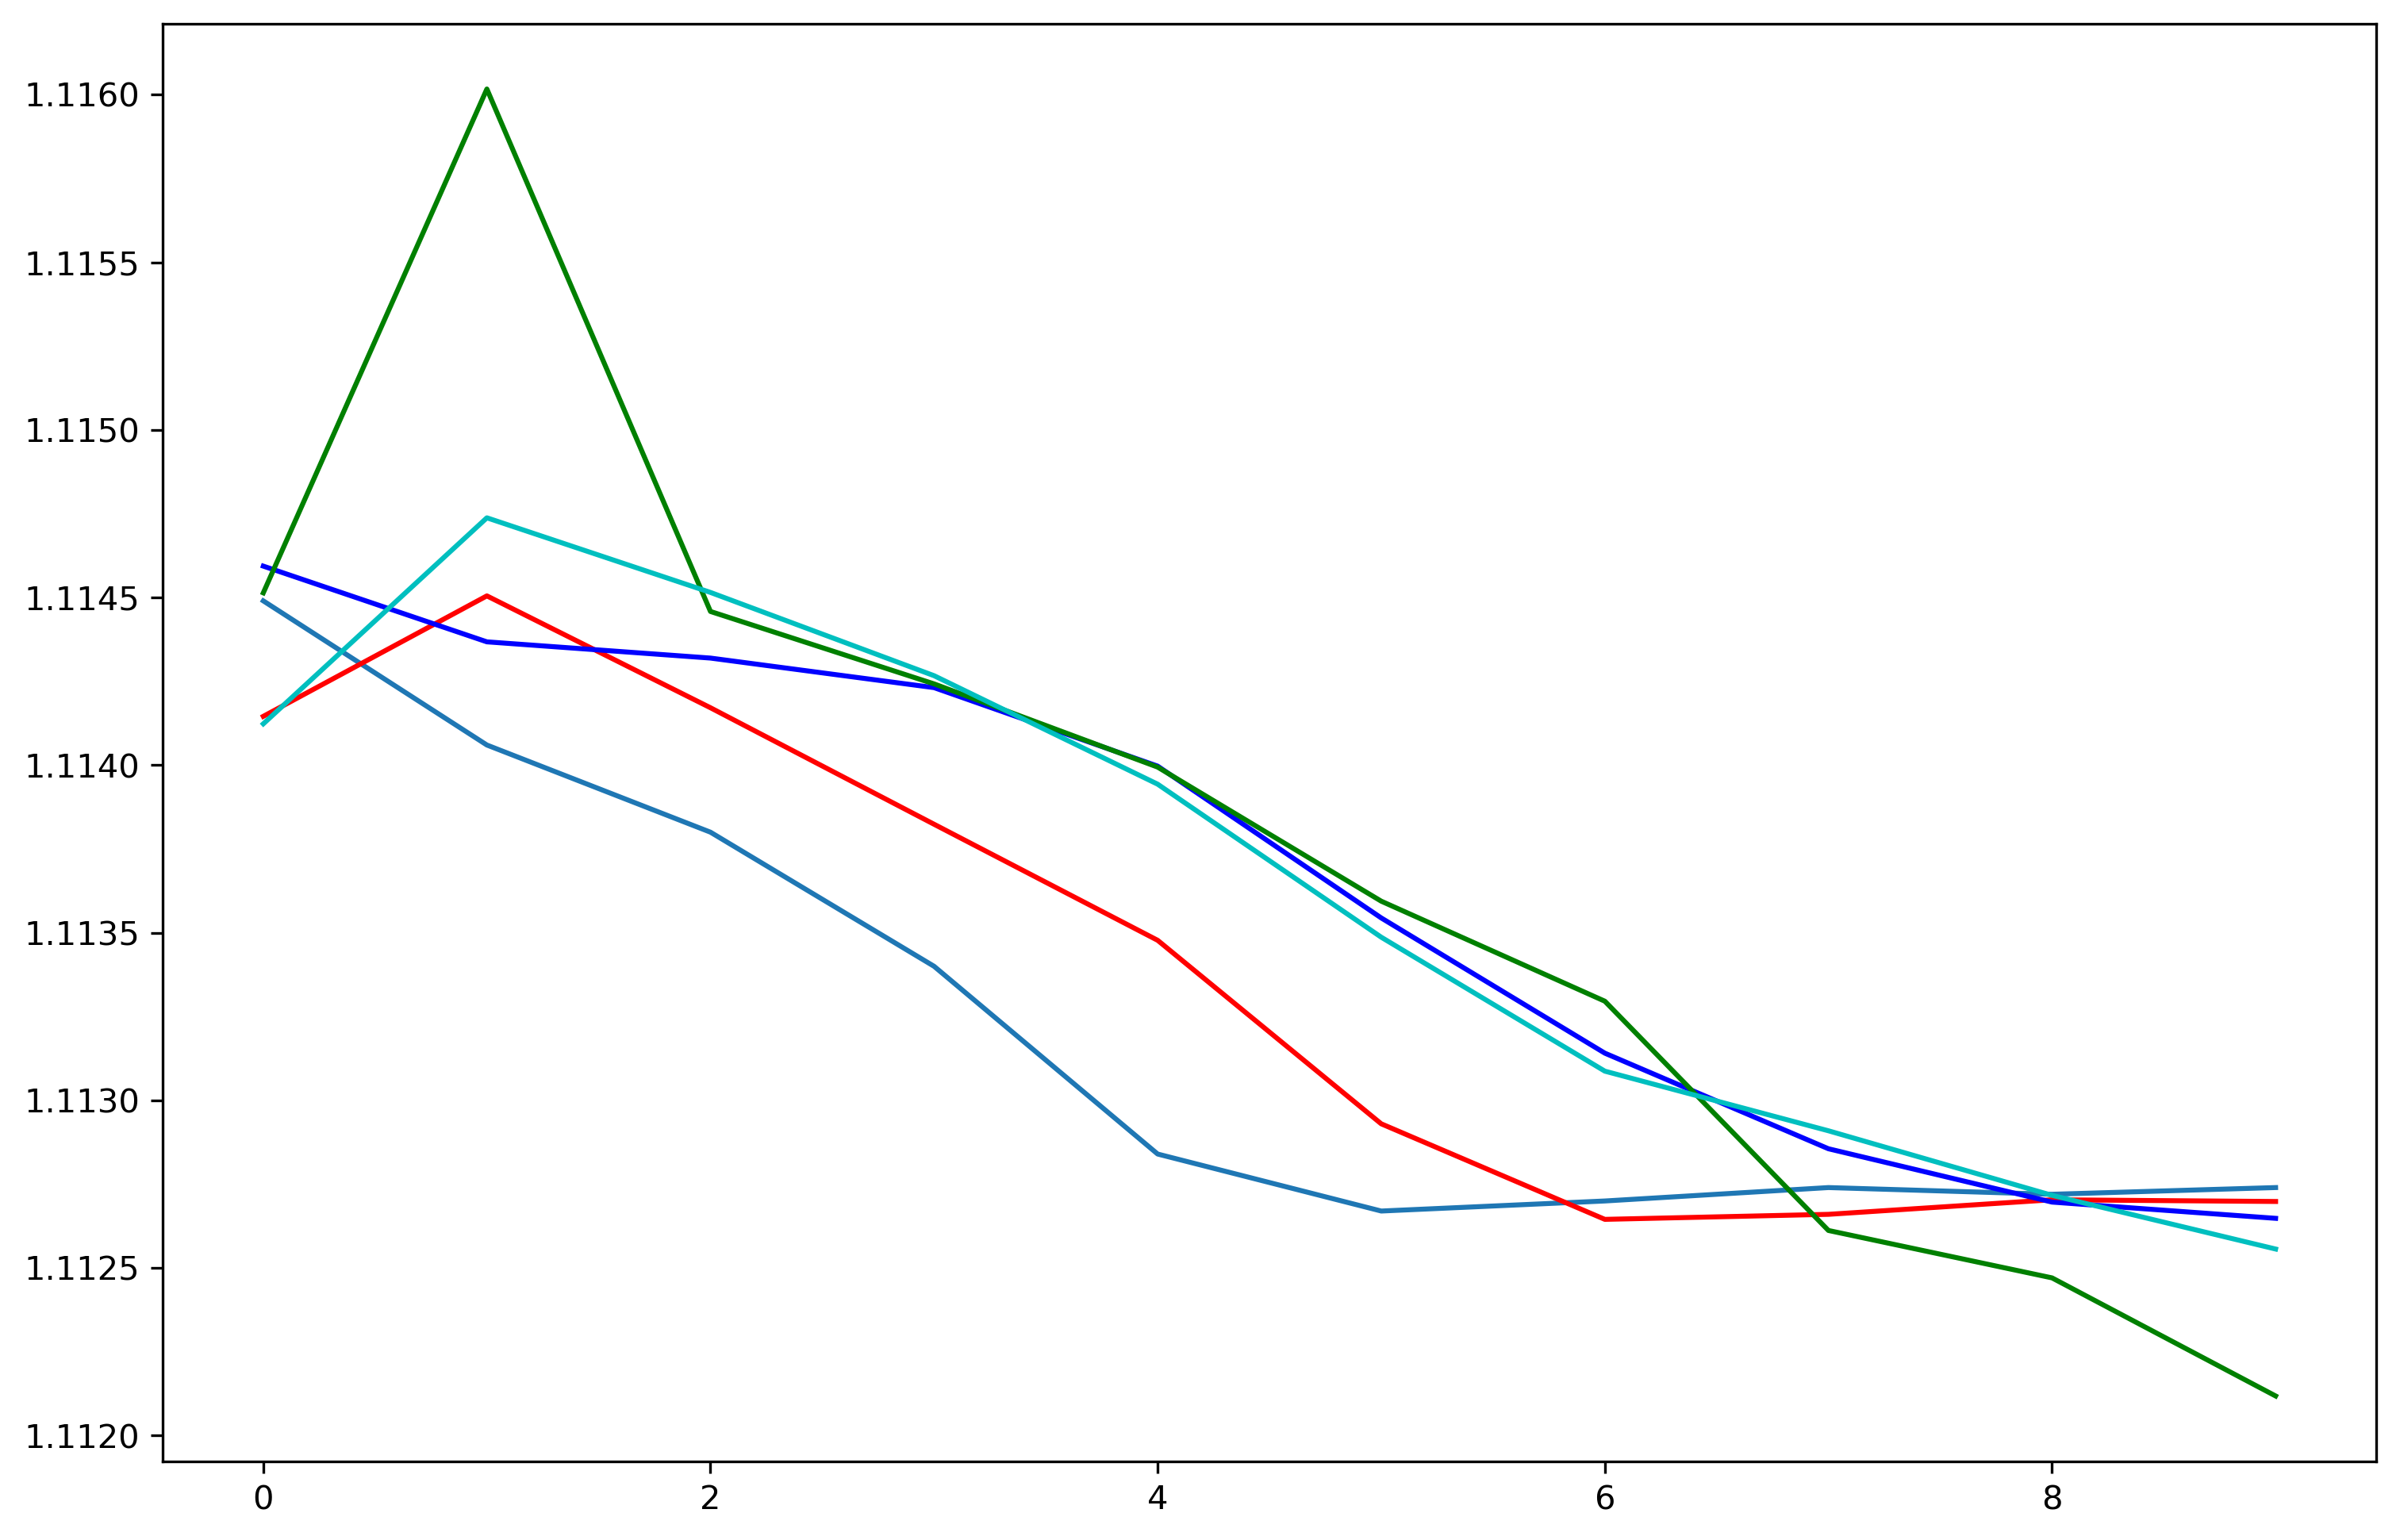
\includegraphics[width=0.7\textwidth]{fig/section3/m30_h1_all_together.png}
\centering 
\caption{Predicted result of last 10 data points with sampling frequency as 30 min and stride as 1. The light blue line is the true data point, the red line corresponded to the predicted result of ARIMA model, the blue, green and cyan lines corresponded to the predicted results of Periodic+Liner kernel, Periodic+RBF kernel, and Periodic+poly kernel models.}
\label{fig:grammar}
\end{figure}

\begin{figure}[H]
\centering 
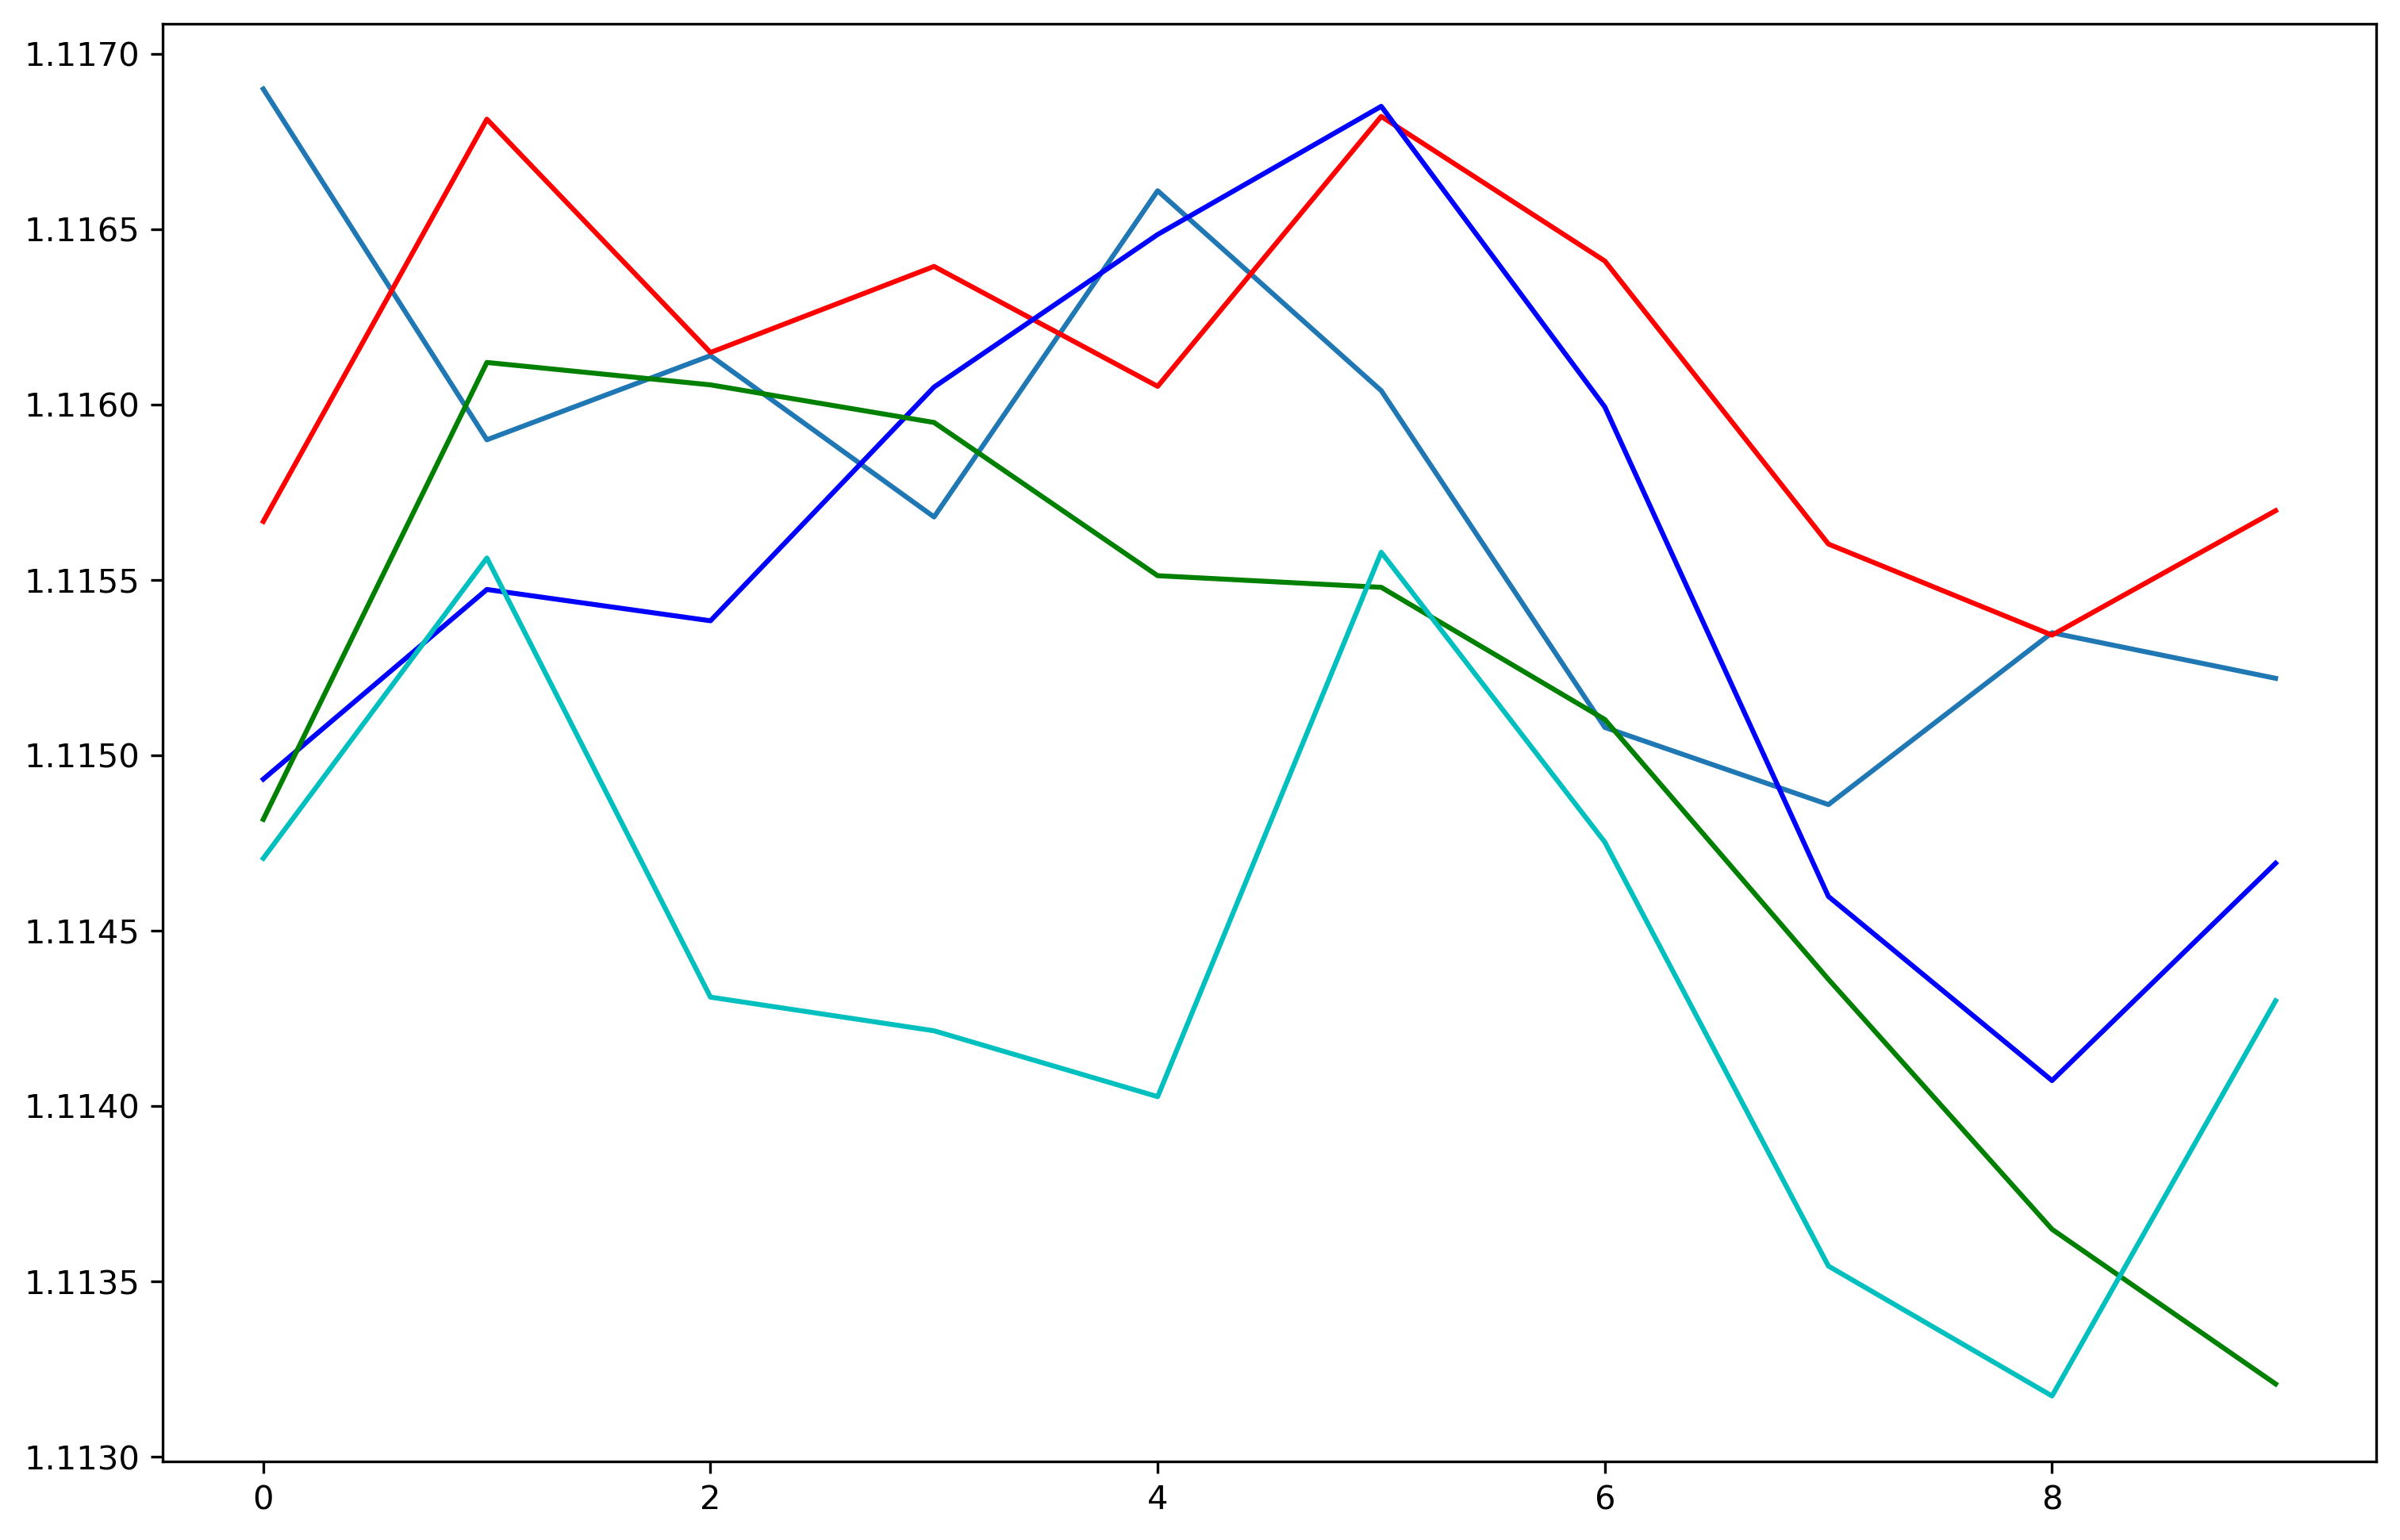
\includegraphics[width=0.7\textwidth]{fig/section3/h4_h1_all_together.png}
\centering 
\caption{Predicted result of last 10 data points with sampling frequency as 4 hours and stride as 1. The light blue line is the true data point, the red line corresponded to the predicted result of ARIMA model, the blue, green and cyan lines corresponded to the predicted results of Periodic+Liner kernel, Periodic+RBF kernel, and Periodic+poly kernel models.}
\label{fig:grammar}
\end{figure}

\begin{table}[H]
\centering
\begin{tabular}{|c|c|c|c|c|}
\hline
Model                 & 1 min             & 5 min             & 30 min            & 4 h              \\ \hline
ARIMA                 & 0.000052          & 0.000151          & 0.000743          & 0.00071          \\ \hline
Periodic+Liner kernel & \textbf{0.000034} & \textbf{0.00009}  & \textbf{0.000446} & \textbf{0.00070} \\ \hline
Periodic+RBF kernel   & \textbf{0.000045} & \textbf{0.000111} & \textbf{0.000715} & 0.00086          \\ \hline
Periodic+poly kernel  & \textbf{0.000036} & 0.000176          & \textbf{0.000529} & 0.0014           \\ \hline
\end{tabular}
\caption{MAE results for 4 different frequencies and 4 models with stride as 1}
\end{table}


Then we set a bigger stride to see the long-term prediction of ARIMA model and GP models. We use the dataset with the longest frequency which is 4 hours and set the stride as 10. Figure 8 shows the predicted result, and table 2 shows the corresponded MAE of different models. We can find that when the stride is 10, the GP model with Periodic+poly kernel outperforms the ARIMA model, which indicates that GP model has better performance than ARIMA in the long-term prediction.



\begin{figure}[H]
\centering 
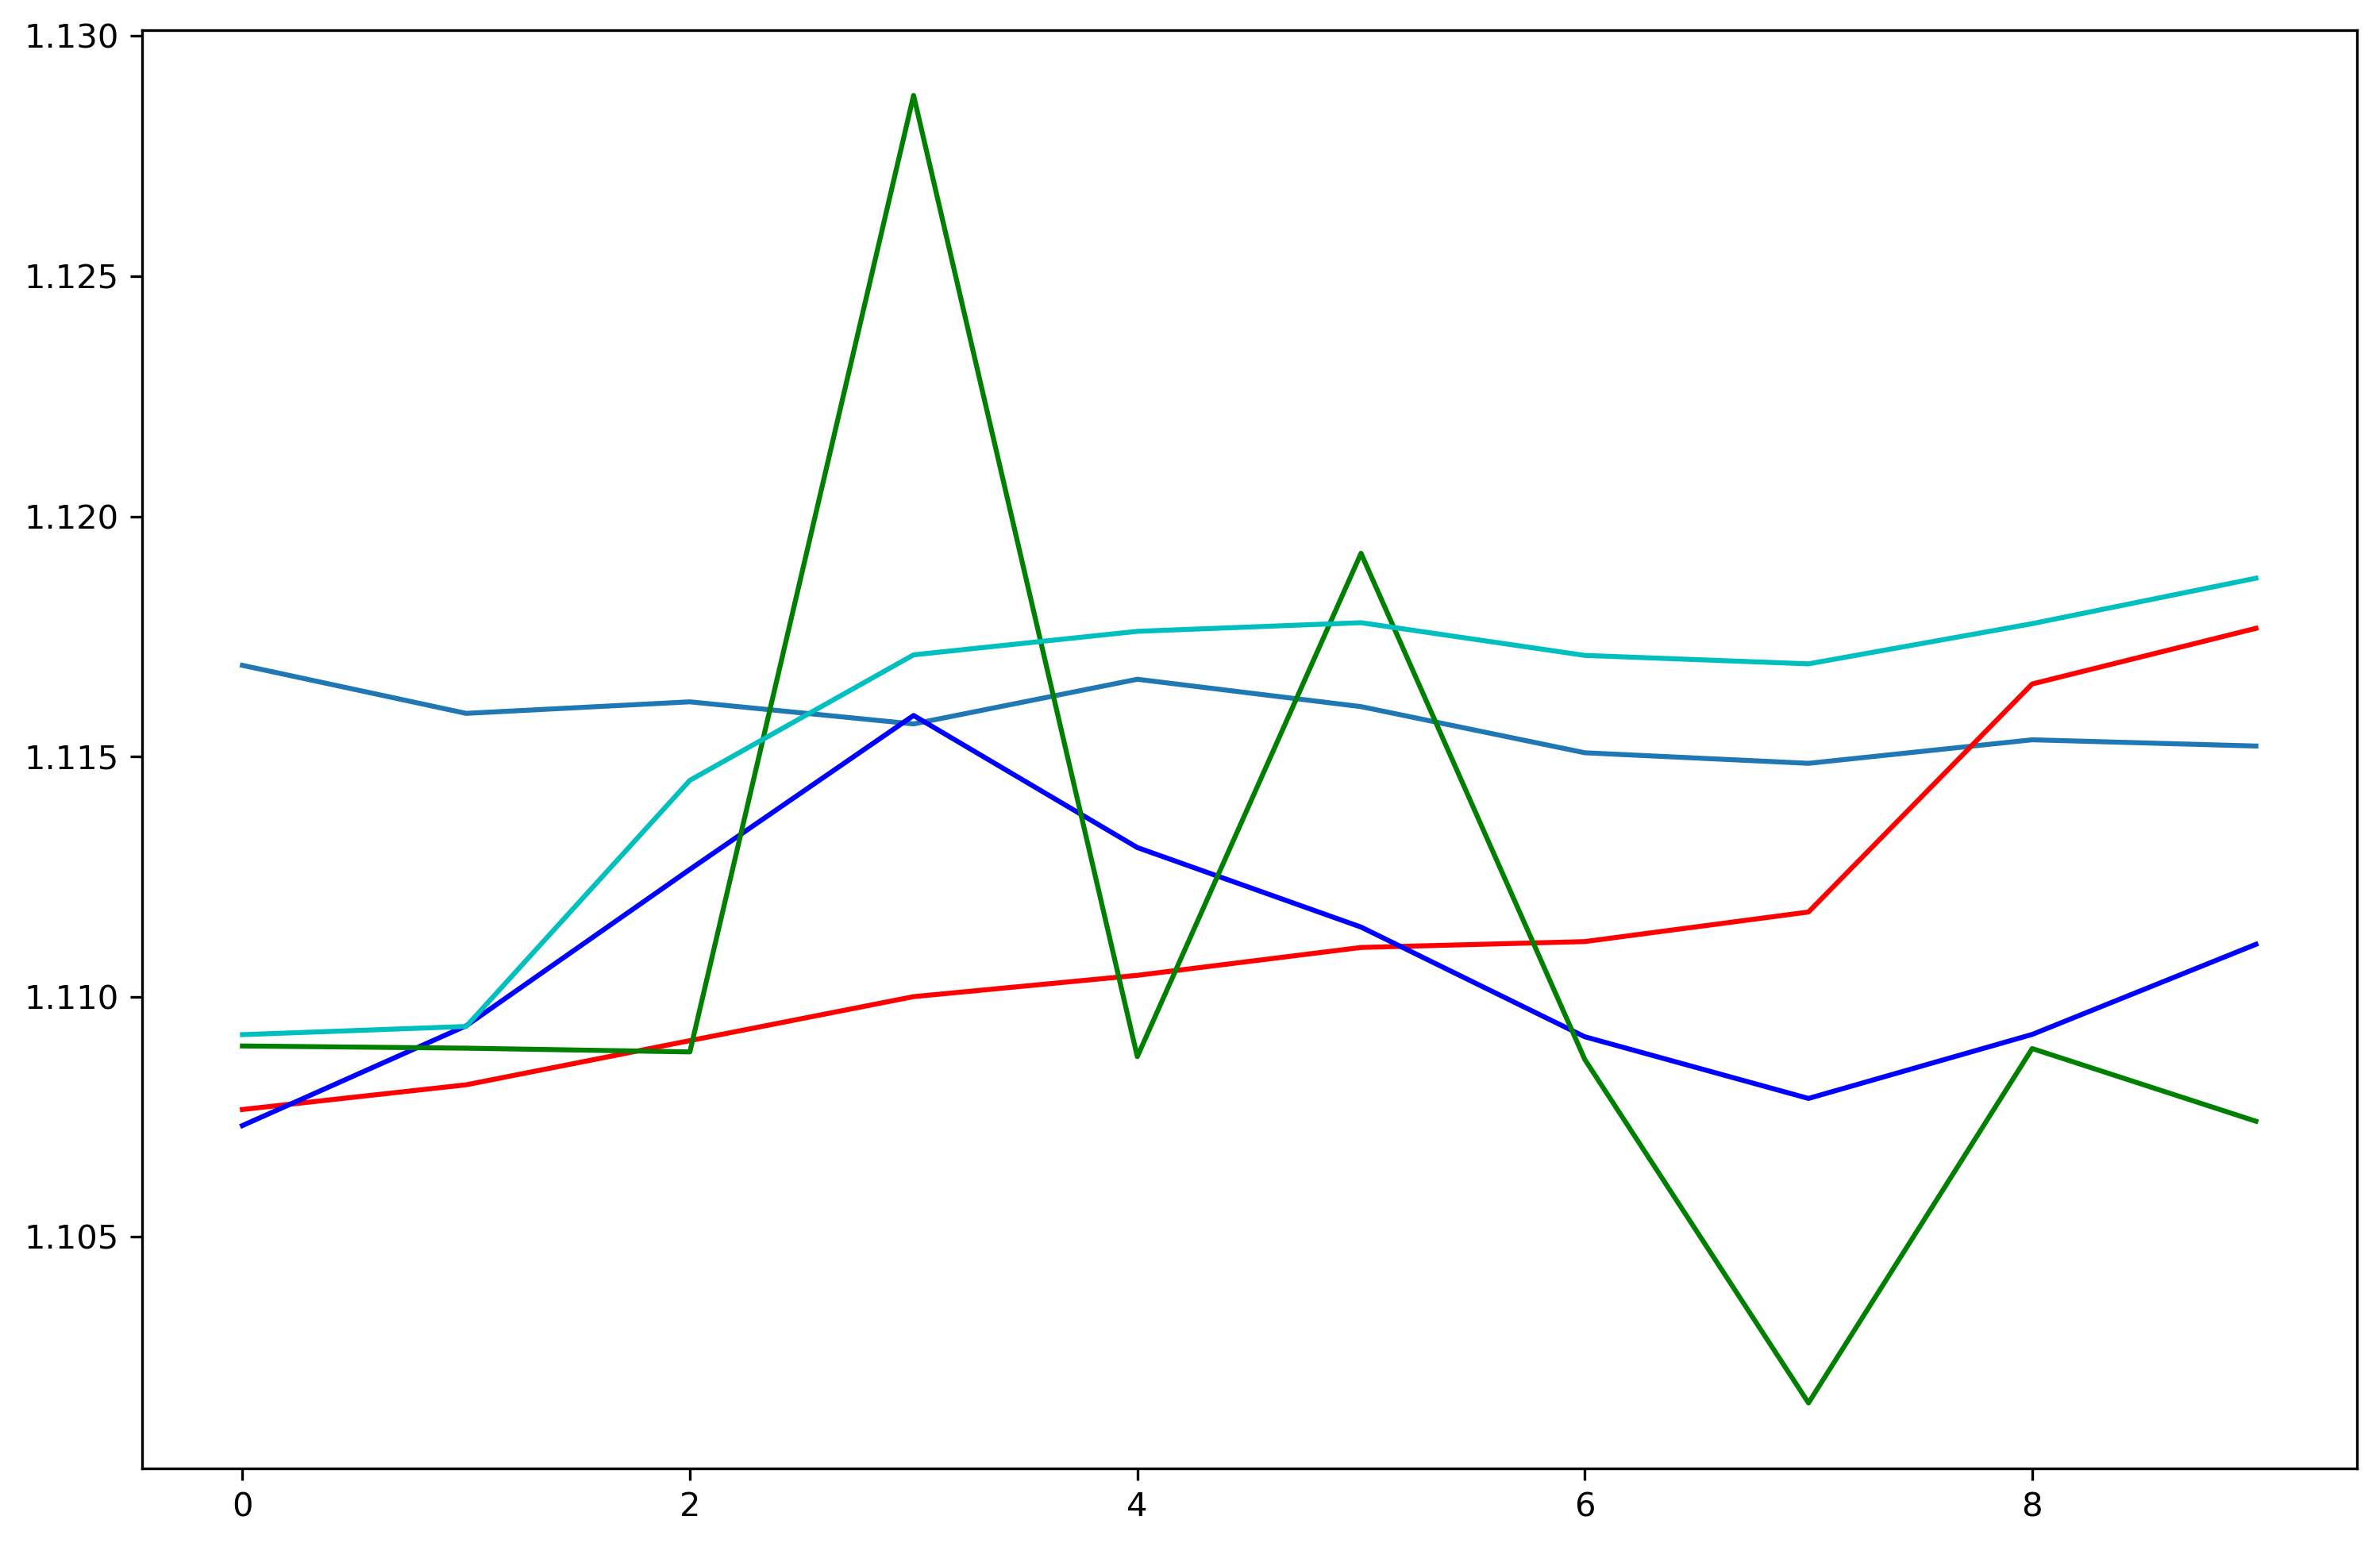
\includegraphics[width=0.7\textwidth]{fig/section3/h4_h10_all_together.png}
\centering 
\caption{Predicted result of last 10 data points with sampling frequency as 4 hours and stride as 10. The light blue line is the true data point, the red line corresponded to the predicted result of ARIMA model, the blue, green and cyan lines corresponded to the predicted results of Periodic+Liner kernel, Periodic+RBF kernel, and Periodic+poly kernel models.}
\label{fig:grammar}
\end{figure}



\begin{table}[H]
\centering
\begin{tabular}{|l|l|l|}
\hline
Models                      & h = 1            & h = 10           \\ \hline
ARIMA                 & 0.00071          & 0.00497          \\ \hline
Periodic+Liner kernel & \textbf{0.00070} & 0.00501          \\ \hline
Periodic+RBF kernel   & 0.00086          & 0.00802          \\ \hline
Periodic+poly kernel  & 0.0014           & \textbf{0.00300} \\ \hline
\end{tabular}
\caption{MAE results of 4 models with frequency as 4 hour and stride as 1 and 10}
\end{table} 

\subsection{Conclusion}
In this experiment, we compared the ARIMA model with three GP models on the datasets with 4 different sampling frequency, the kernels of the three GP models are Periodic+Liner kernel, Periodic+RBF kernel, and Periodic+poly kernel, respectively. We used a walk-forward validation method to evaluate model performance, and we also used 2 prediction strides to see the model performance on short-term and long-term predictions. 
We found that by choosing suitable kernels, GP model can always perform better than ARIMA, especially for the long-term prediction.





\section{From Gaussian Process to Kalman Filter}

\subsection{Kalman Filter}
Despite the good performance of Gaussian Processes, computationally it is not conveniently for long (or unbounded) time-series. For certain covariance functions, the Gaussian process can be represented as a state space model\cite{sarkka:2010:kalmanfilter}. It solves problems on the given dataset $\{(x_i,y_i)\}_{i=1}^n$ :
\begin{equation}
    \begin{split}
     &\bm{f}(x_k)\sim N(\bm{f}(x_k)|\bm{A}_{k-1}\bm{f}(x_{k-1}),\bm{Q}_{k-1}) \\
     &y(x_k)\sim N(y(x_k)|\bm{H_k}\bm{f}(x_k),\sigma_{noise}^2)
\end{split}
\label{eq:discrete SDE}
\end{equation}
where $\bm{A}_k$ is the discrete-time state transition matrix between $x_k$ and $x_{k-1}$, $\bm{Q}_k$ is the process noise covariance matrix, $\bm{H_k}$ is the measurement model matrix.\\ 

Kalman filter \cite{kalman:1960:kalmanfilter} is a closed form solution to the state space model (\ref{eq:discrete SDE}), where the dynamic and measurement models are linear Gaussian, and the resulting distributions are Gaussian. It could evaluate the likelihood function associated with the state
space model.\\


\subsection{Comparison Between Gaussian Process and Kalman Filter}
In this section we compared various performance of Gaussian Process and kalman filter with martern32 kernel on the same trading dataset, using the sliding window method. We will show that kalman filter can run much faster than GP, while keep the performance of mean absolute error and model fitness almost the same. Also, we implemented the real-time online predictioin with GP by updating the dataset with the API, and it worked quite well (Kalman filter should be the same).

\subsubsection{Offline predict}
Here we use the downloaded offline dataset and predict the trading value using sliding window method. The sampling frequency is 1 min, which is the smallest frequency that we can get from the fxcmpy API. Figure 4.1 shows the example of the trading dataset. In the following examples, the sliding window move step is 1; the training data length is 100, and the predict length is 10.\\

We implemented the Gaussian process regression and Kalman filter on the same traing and test dataset, the prediction result are shown in figure 4.1 and figure 4.2. Here we show the details of the comparison: Mean log likelihood of kalman filter is: 803.23, while the mean log likelihood of GP is: 787.78; Mean computing time of kalman filter is: 20.85 milliseconds, while the mean computing time of GP is: 619.99 milliseconds; Mean absolute error for prediction of kalman filter is: 4.62e-05, while the mean absolute error for prediction of GP is: 5.58e-05. From the result, we can see that kalman filter can run much faster than GP, while keep the performance of mean absolute error and model fitness almost the same. 


\begin{figure}[H]
\centering 
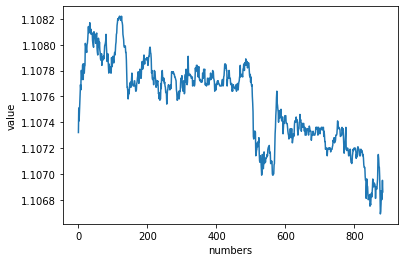
\includegraphics[width=0.7\textwidth]{fig/section4/example.png}
\caption{example of dataset}
\end{figure}

\begin{figure}[H]
\centering 
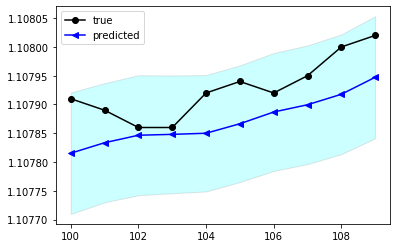
\includegraphics[width=0.7\textwidth]{fig/section4/GPoffline.png}
\caption{GP offline}
\end{figure}


\begin{figure}[H]
\centering 
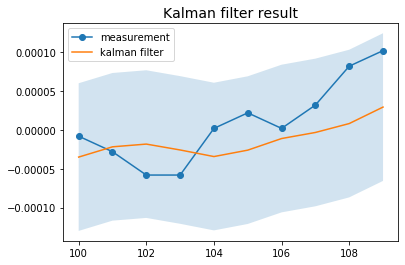
\includegraphics[width=0.7\textwidth]{fig/section4/KFoffline.png}
\caption{KF offline}
\end{figure}


\subsubsection{Online predict}
Here we use the fxcmpy API to download the trading data and predict the trading value. We only showed the implementation of GP, and kalman filter should be the same as GP. Still, the frequency of trading data is 1 min, so we download the new data every 1 min. Also, the sliding window step is 1, the training data length is 100, and the predict length is 10, which are the same as offline prediction. Figure 4.3 shows the example of online prediction using GP. The mean computing time for each step is: 248 milliseconds, and mean absolute error for the prediction is 0.0006. 

\begin{figure}[H]
\centering 
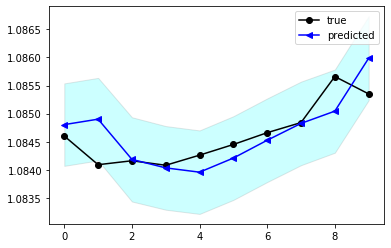
\includegraphics[width=0.7\textwidth]{fig/section4/GPonline.png}
\centering 
\caption{GP online}
% \label{fig:grammar}
\end{figure}


\pagebreak
\printbibliography

\newpage
\begin{appendices}


\end{appendices}

\end{document}
